\section{Effects of Noise on Speaker Adaptation}
\label{noise_speaker_adaptation}
Adapting from an average voice model is an efficient way of dealing with limited amount of data.
%
Using the noisy data in the adaptation allows us to use a smaller amount of data corrupted than the needed if we use it in building a model starting from scratch.
%
Therefore, less feature vectors corrupted by noise are used to estimate the final models.

Noise present in the adaptation data can add background noise to the synthetic speech or reduce its naturalness or similarity compared to adaptation done with clean data \cite{karhila_jstsp_14}.
%
Depending on the vocoder used, the behavior displayed by the system may vary.

Previously, the speaker-adaptive HMM-based speech synthesis paradigm has been found to be quite robust on mel-cepstrum \cite{karhila_jstsp_14, yamagishi2008robustness} and Mel-LSP \cite{Yanagisawa_SSW8} based vocoders.
%
In this work we focus on the GlottHMM vocoder and compare it to the STRAIGHT vocoder.
%
Both vocoders model the excitation of the voice differently.
%
The GlottHMM estimates glottal pulse via inverse filtering while STRAIGHT features pitch-adaptive extraction of spectrum (see Section \ref{vocoders}).

Environmental noise can interfere with speech, as not all kind of noises can be filtered out of the signal without damaging the speech.
%
Specially, noise signals that are time (and frequency) variant and occupy the same frequency bands provides the most difficult and challenging cases.
%
When the noise cannot be removed the system must tolerate it.
%
In this project three different noises are studied: babble, factory and machine gun noises.
%
Among them, the most interesting one is the babble noise, because of its similar nature with speech and because it is the more common noise present when recording speech, as usually factories or environments involving gunfire are not chosen for, for example, interviewing people.
%
As this is the most interesting case, the comparison between the GlottHMM and STRAIGHT vocoders is done for these cases.

Parametric vocoders represent the complete spectrum in some dozens of parameters.
%
The ability to focus on the speech signal and smooth out the extra noise varies between vocoders.

\begin{figure}[!htb]
\begin{centering}
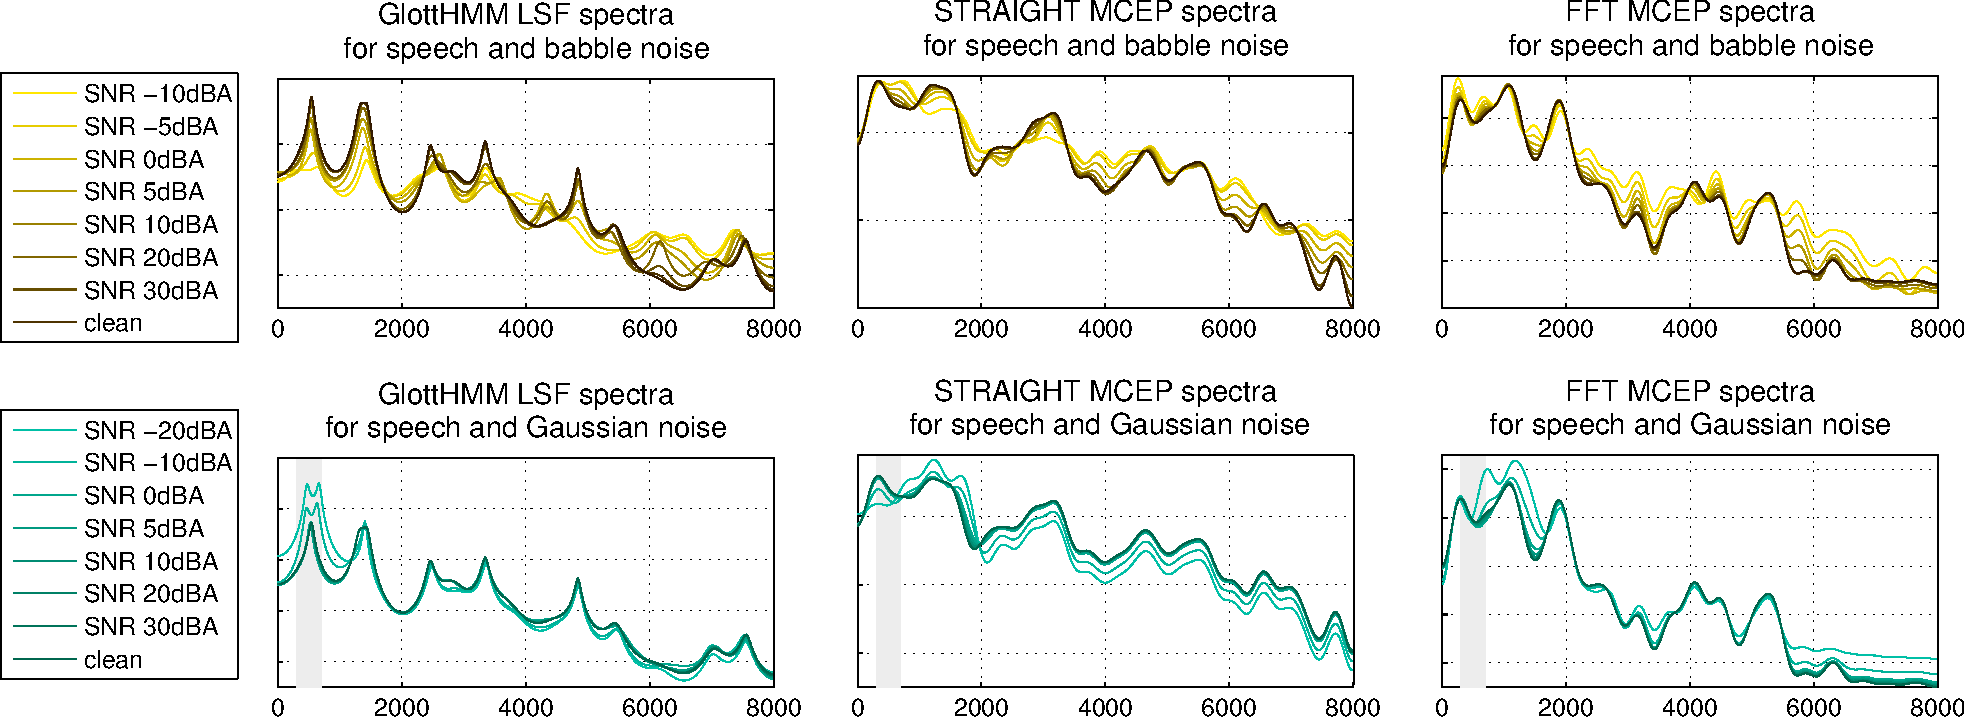
\includegraphics[width=\textwidth]{images/vowel_frame_and_noise_w_fft.pdf}
\caption{Spectra for GlottHMM LSF (left), STRAIGHT MCEP components (middle) and FFT MCEP components (right) of a male speaker's vowel frame, with added babble (top) or band-limited Gaussian noise in the 300-700 Hz frequency band (bottom), shown in the figures in grey \cite{moreno_interspeech}}
\label{fig:different_specs_noise}
\end{centering}
\end{figure}

Figure \ref{fig:different_specs_noise} shows how GlottHMM, STRAIGHT and the standard Fast Fourier Transform (FFT) react to vowel frames with added babble and Gaussian band-limited noise.
%
It is obvious that all vocoders tolerate moderate amounts of Gaussian noise.
%
Looking at the GlottHMM graphs, it can be seen that LSF models are locally affected by increased noise.
%
The noise masks the speech signal locally reducing the accuracy of the LSF components in the area and even causing the formation of extra peaks.
%
In the case of Gaussian noise, no effects are spotted out of the region where the noise was added. 

If we look at the STRAIGHT graphs, the effects of the added Gaussian noise are more widely spread.
%
The energy of the signal is redistribution with the decrease of the SNR, maintaining the shape of the spectral envelope in the higher frequency range although it is shifted.
%
The effect of the noise is seen up to the 2000 Hz region.
%

As comparison, in the FFT spectra the effects of the Gaussian noise can be spotted up to the 1500 Hz region.
%
However, the rest of the spectrum remains largely without effect, except the higher frequencies, where the envelope is raised due to the jitter of the Gaussian noise.

On the other hand, the effects due to babble noise are very clear for all the vocoders.
%
Valleys and peaks are moved and specially the LSF spectra shows more severe effects than the other two, with the appearance of sharp new peaks in mid and high frequencies.

\begin{table}[!htb]
\begin{centering}
\begin{tabular}{c c|c c|c c|c c}
	 & & \multicolumn{2}{c|}{Original} & \multicolumn{2}{c|}{GlotHMM} & \multicolumn{2}{c}{STRAIGHT}\\
	 & & \multicolumn{2}{c|}{training} & \multicolumn{2}{c|}{resynth.} & \multicolumn{2}{c}{resynt.}\\
	 & & \multicolumn{2}{c|}{data} & \multicolumn{2}{c|}{data} & \multicolumn{2}{c}{data}\\
	Noise & SNR & fwS & MCD & fwS & MCD & fwS & MCD\\
	\midrule
	\midrule
	\multirow{2}{*}{Clean} & \multirow{2}{*}{-} & \multirow{2}{*}{35.0} & \multirow{2}{*}{0.0} & 14.6 & 1.0 & \multirow{2}{*}{15.5} & \multirow{2}{*}{1.5}\\
	 & & & & 15.9 & 2.1 & & \\	
	\midrule
	\multirow{3}{*}{Babble} & 20 & 20.7 & 1.1 & 15.6 & 2.3 & 14.0 & 2.0\\
	 & 10 & 12.9 & 2.0 & 10.3 & 2.1 & 10.7 & 3.0\\
	 & 5 & 9.5 & 2.5 & 8.3 & 2.5 & 8.4 & 3.4\\
	\midrule
	\midrule
	\multirow{2}{*}{Enhanced} & 20 & 20.7 & 1.1 & 15.7 & 2.3 & 14.1 & 2.0\\
	\multirow{2}{*}{Babble} & 10 & 13.3 & 1.8 & 11.3 & 2.1 & 11.0 & 2.6\\
	 & 5 & 10.1 & 2.2 & 8.8 & 2.2 & 9.1 & 3.1\\
	\bottomrule
\end{tabular}
\caption{Averaged fwSNRseg and MCD measures for 3 speakers. For the GlottHMM vocoder in clean conditions two results are shown: the below one uses the noise reduction system. All noise-affected systems use the noise reduction mechanism. The STRAIGHT values were calculated in \cite{karhila_jstsp_14}}
\label{table:an_resyn_results}
\end{centering}
\end{table}

The effects of babble noise are illustrated in Table \ref{table:an_resyn_results}, where the fwSNRseg and MCD results (see Section \ref{evaluation}) for three test speakers' data analyzed and resynthesized with both GlottHMM and STRAIGHT vocoders are shown.
%
For reference, the results of the original audio recordings are also shown.
%
For GlottHMM in clean conditions two different results are shown: the first one does not use the noise reduction module (see Appendix \ref{glott_conf_noise_red}) and the second one is obtained using it.
%
The SNR measures show that GlottHMM is able to reproduce the speech signal when the SNR is high enough, but the quality drops rapidly when the SNR of the signals gets low.
%
It is very interesting that the MCD scores for GlottHMM do not behave as they are expected to.
%
A noisier case (babble 10dB) is judge to be better than a cleaner one (babble 20dB).
%
The performance obtained with STRAIGHT is the expected.
%
Noisier cases are rated as lower quality cases by the two different measures.

The performance of the GlottHMM vocoder according to different values of the noise reduction parameters is investigated in Section \ref{experiments_initial}.